
\begin{figure}[h]
	\centering
	\begin{subfigure}[b]{0.49\textwidth}
        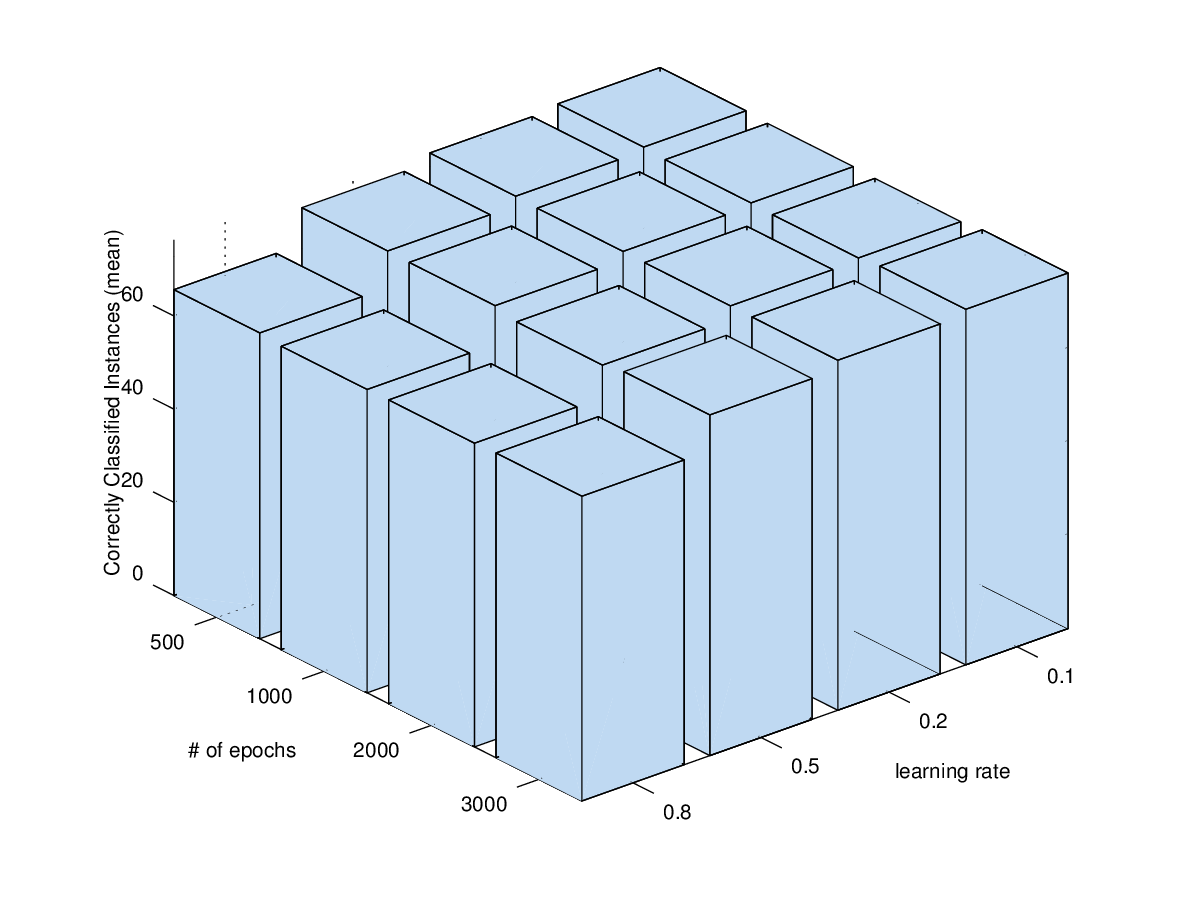
\includegraphics[width=\textwidth]{plots/cmean_NL.png}
        \caption{Escala lineal.}
        \label{fig:cmean_NL-lin}
    \end{subfigure}
	\begin{subfigure}[b]{0.49\textwidth}
        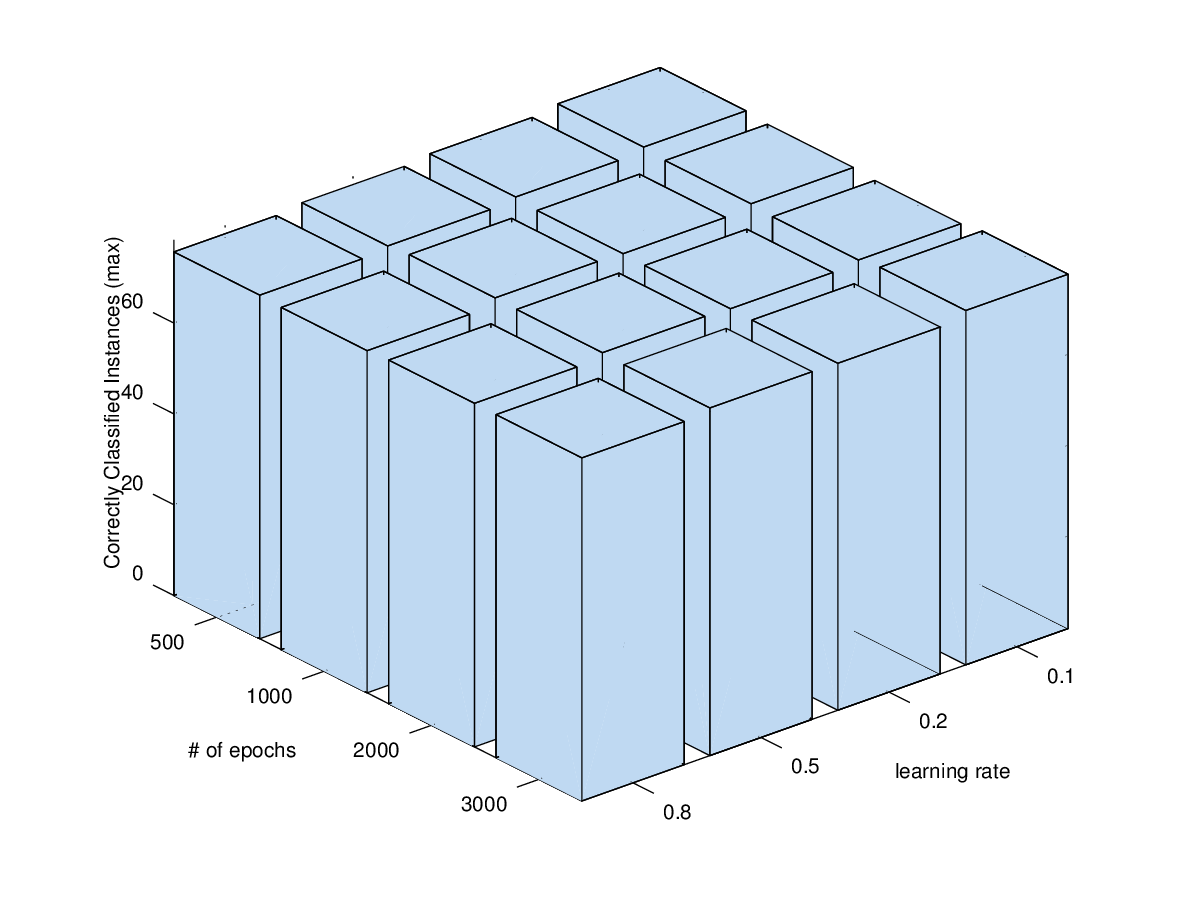
\includegraphics[width=\textwidth]{plots/cmax_NL.png}
        \caption{Escala lineal.}
        \label{fig:cmax_NL-lin}
    \end{subfigure}
    \\
	\begin{subfigure}[b]{0.49\textwidth}
        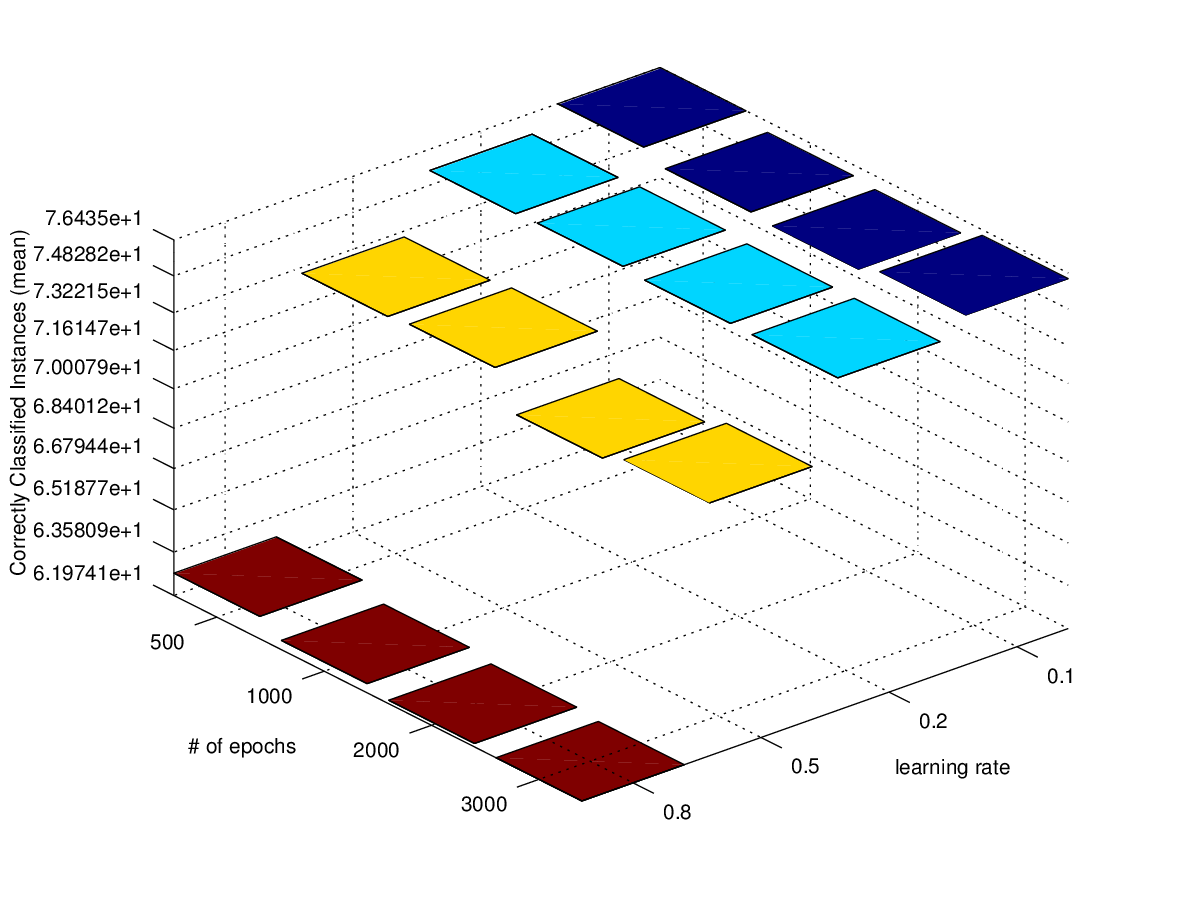
\includegraphics[width=\textwidth]{plots/cmean_NL-log.png}
        \caption{Escala logarítmica.}
        \label{fig:cmean_NL-log}
    \end{subfigure}
	\begin{subfigure}[b]{0.49\textwidth}
        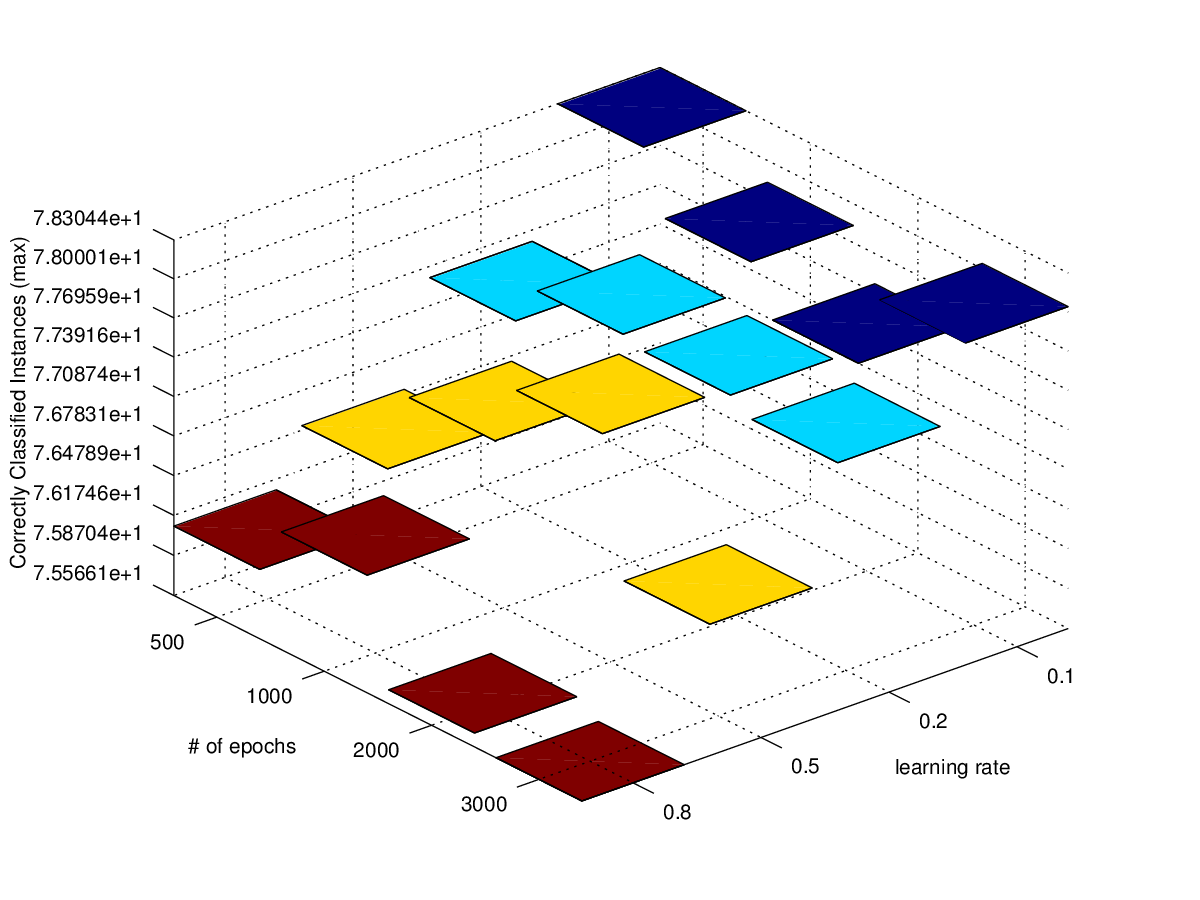
\includegraphics[width=\textwidth]{plots/cmax_NL-log.png}
        \caption{Escala logarítmica.}
        \label{fig:cmax_NL-log}
    \end{subfigure}    
	
	\caption{La proyección del \emph{número de épocas} utilizado y el \emph{``learning rate''} 
			 sobre la \textbf{media} (izquierda: \ref{fig:cmean_NL-lin}, \ref{fig:cmean_NL-log})
			 y el \textbf{máximo} (derecha: \ref{fig:cmax_NL-lin}, \ref{fig:cmax_NL-log})
			 del \emph{número de instancias correctamente clasificadas}. 
			}
	\label{fig:NL}
\end{figure}


\begin{figure}[h]
	\centering
	\begin{subfigure}[b]{0.49\textwidth}
        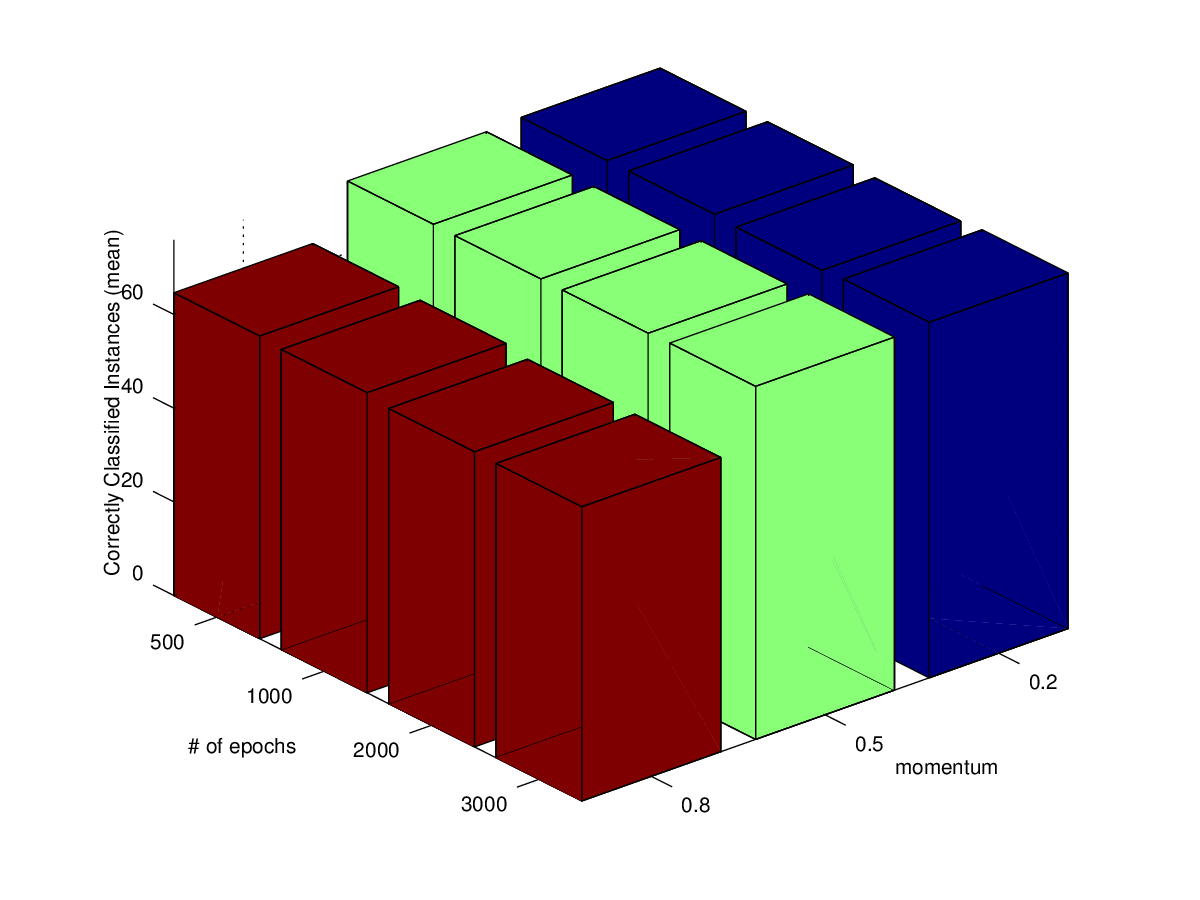
\includegraphics[width=\textwidth]{plots/cmean_NM.png}
        \caption{Escala lineal.}
        \label{fig:cmean_NM-lin}
    \end{subfigure}
	\begin{subfigure}[b]{0.49\textwidth}
        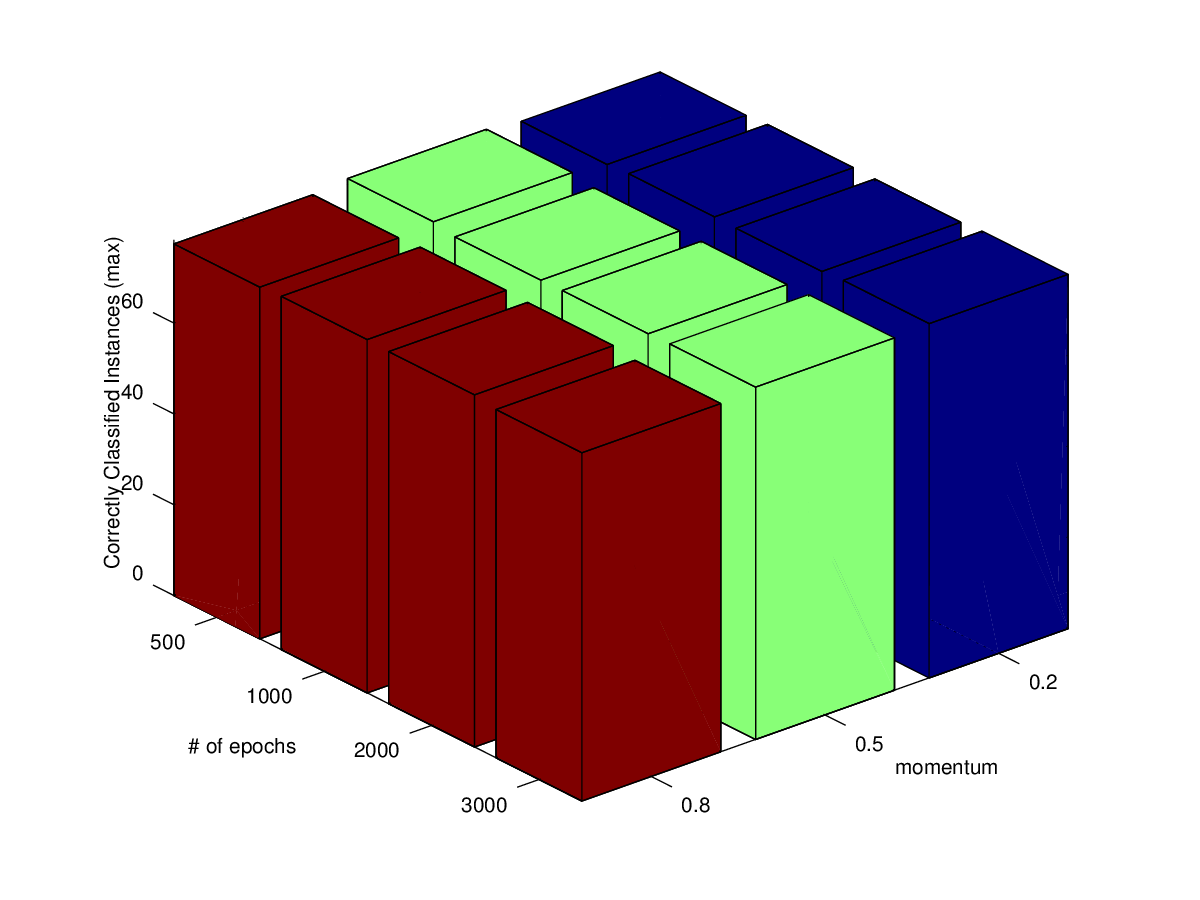
\includegraphics[width=\textwidth]{plots/cmax_NM.png}
        \caption{Escala lineal.}
        \label{fig:cmax_NM-lin}
    \end{subfigure}
    \\
	\begin{subfigure}[b]{0.49\textwidth}
        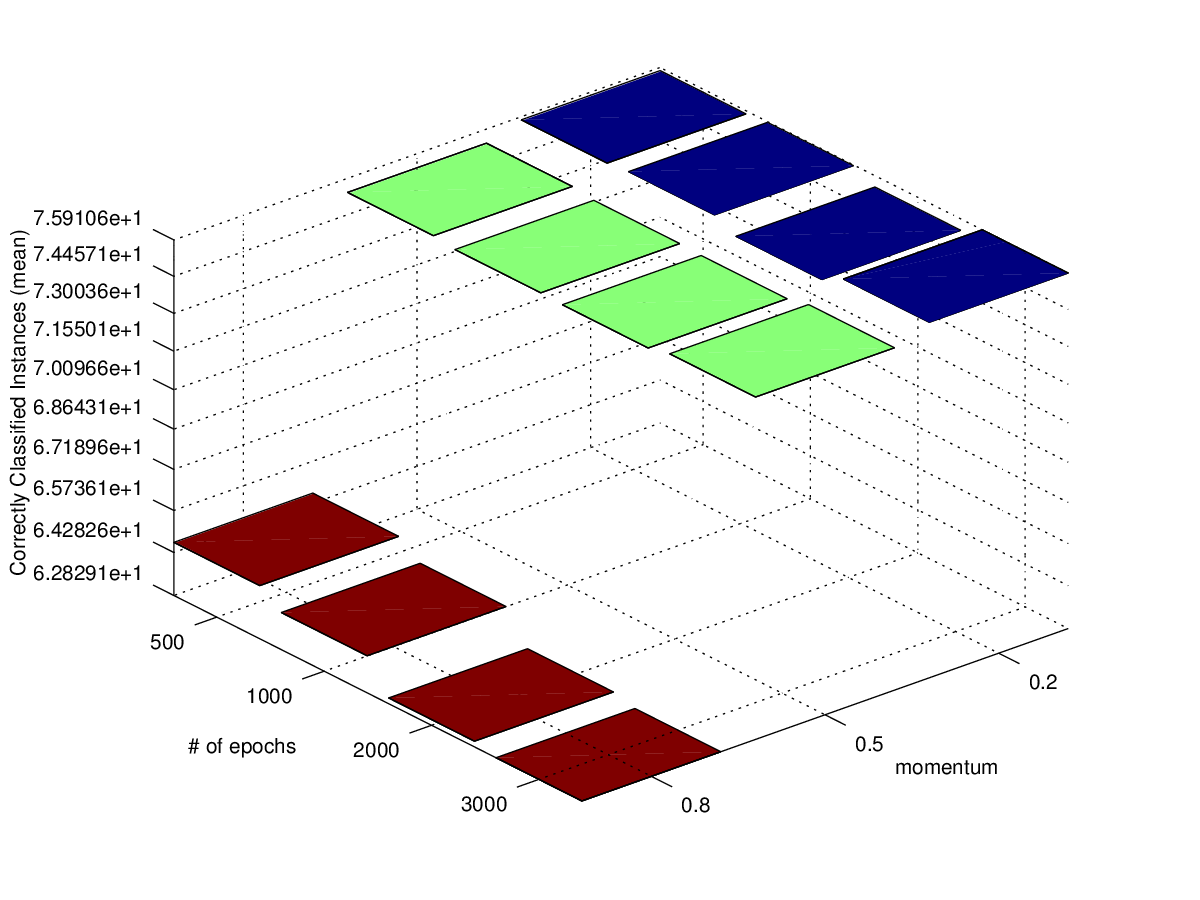
\includegraphics[width=\textwidth]{plots/cmean_NM-log.png}
        \caption{Escala logarítmica.}
        \label{fig:cmean_NM-log}
    \end{subfigure}
	\begin{subfigure}[b]{0.49\textwidth}
        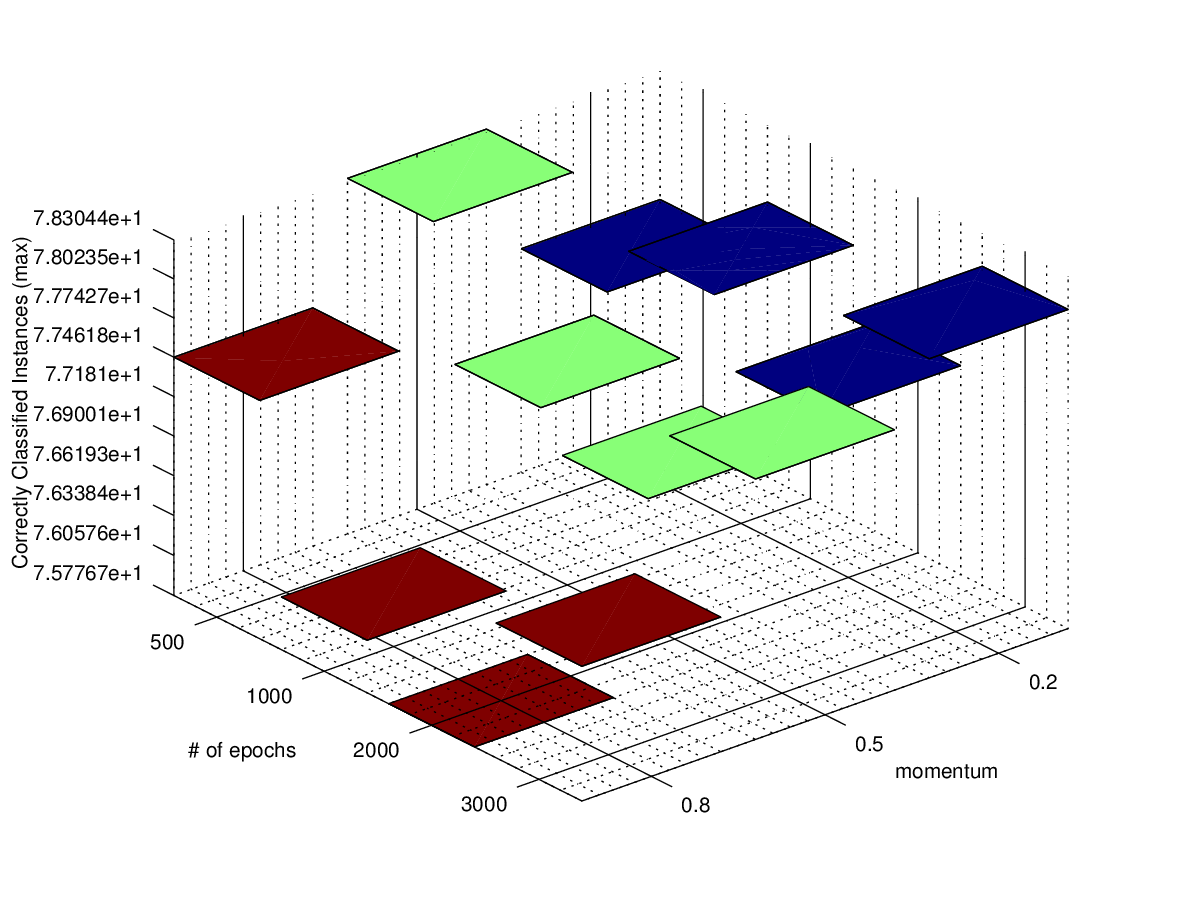
\includegraphics[width=\textwidth]{plots/cmax_NM-log.png}
        \caption{Escala logarítmica.}
        \label{fig:cmax_NM-log}
    \end{subfigure}    
	
	\caption{La proyección del \emph{número de épocas} utilizado y el \emph{``momentum''} 
			 sobre la \textbf{media} \ref{fig:cmean_NM-lin, fig:cmean_NM-log} (izquierda) 
			 y el \textbf{máximo} (derecha) \ref{fig:cmax_NM-lin}, \ref{fig:cmax_NM-log}
			 del \emph{número de instancias correctamente clasificadas}. }
	\label{fig:NM}
\end{figure}

\begin{figure}[h]
	\centering
	\begin{subfigure}[b]{0.49\textwidth}
        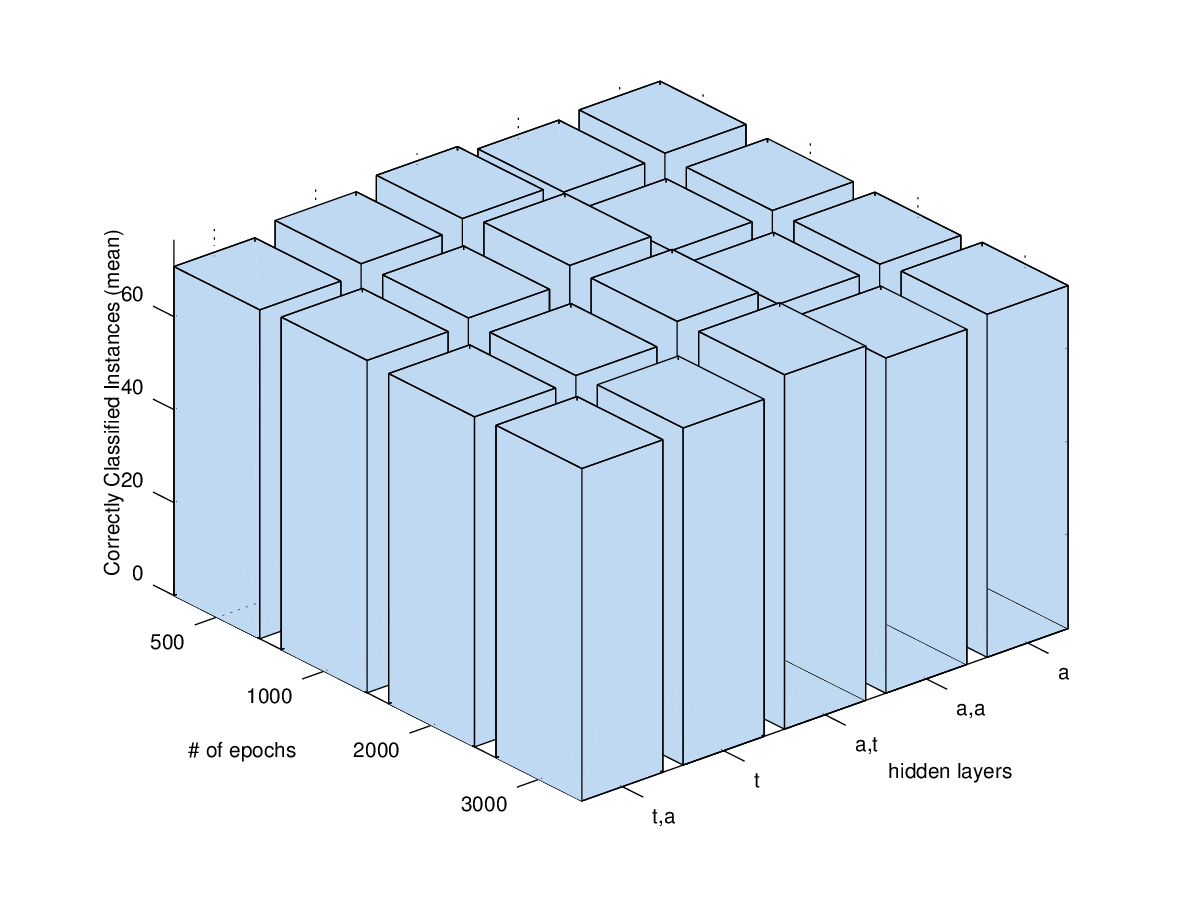
\includegraphics[width=\textwidth]{plots/cmean_NH.png}
        \caption{Escala lineal.}
        \label{fig:cmean_NH-lin}
    \end{subfigure}
	\begin{subfigure}[b]{0.49\textwidth}
        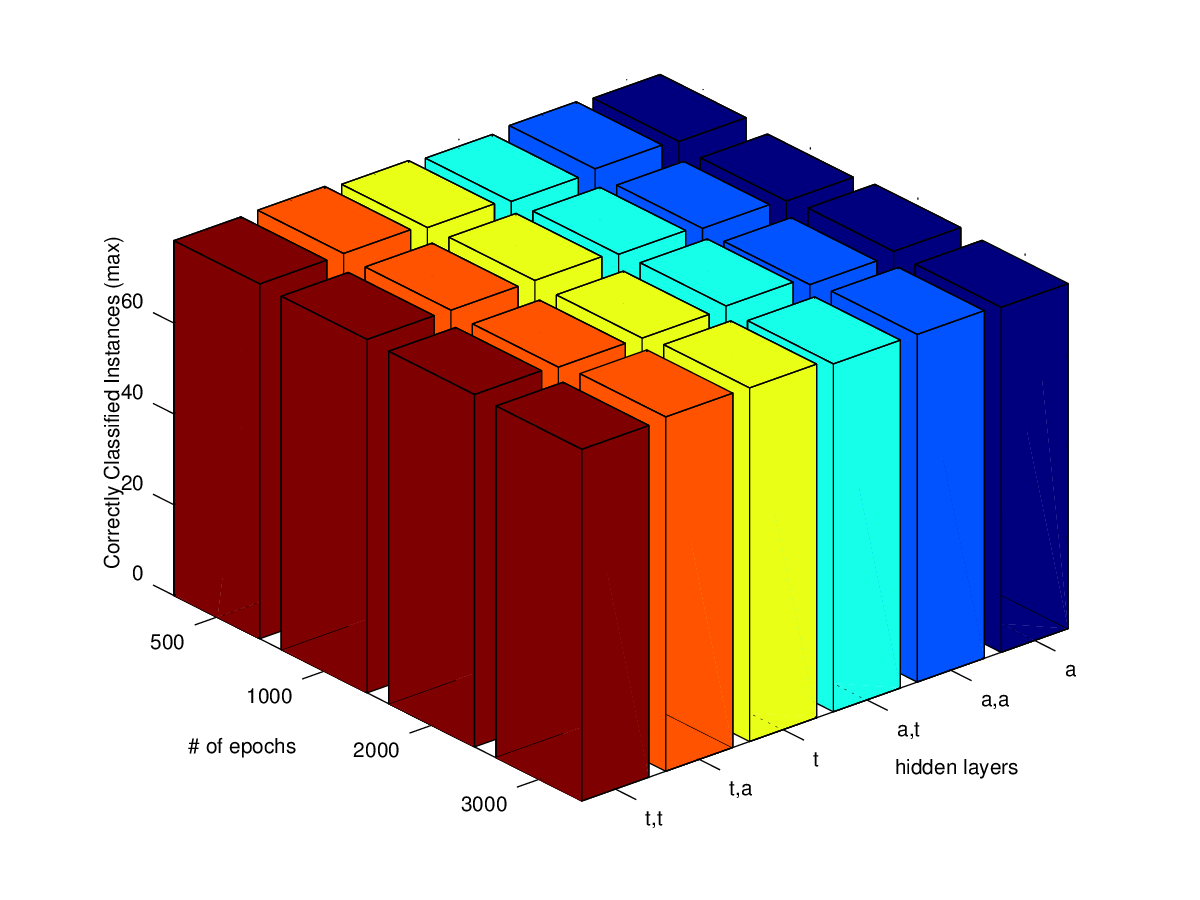
\includegraphics[width=\textwidth]{plots/cmax_NH.png}
        \caption{Escala lineal.}
        \label{fig:cmax_NH-lin}
    \end{subfigure}
    \\
	\begin{subfigure}[b]{0.49\textwidth}
        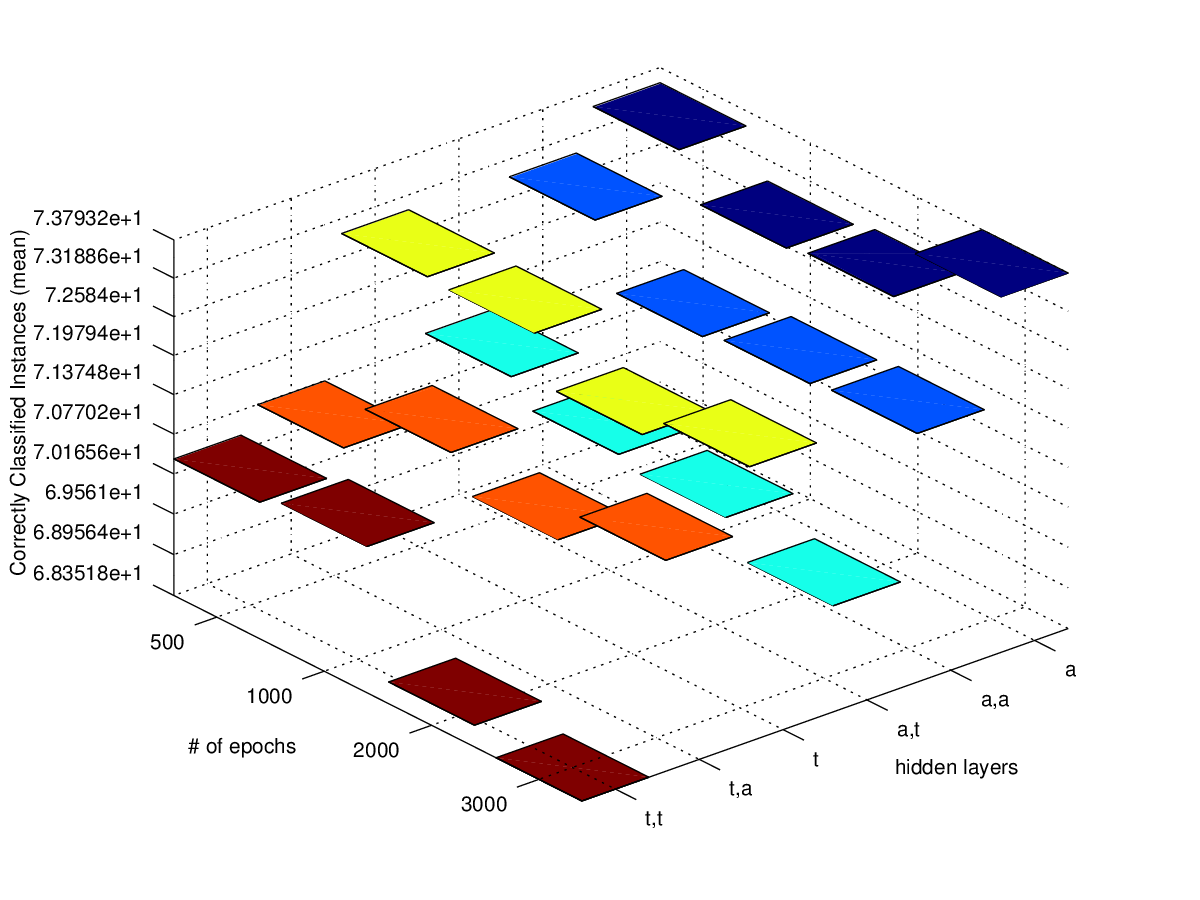
\includegraphics[width=\textwidth]{plots/cmean_NH-log.png}
        \caption{Escala logarítmica.}
        \label{fig:cmean_NH-log}
    \end{subfigure}
	\begin{subfigure}[b]{0.49\textwidth}
        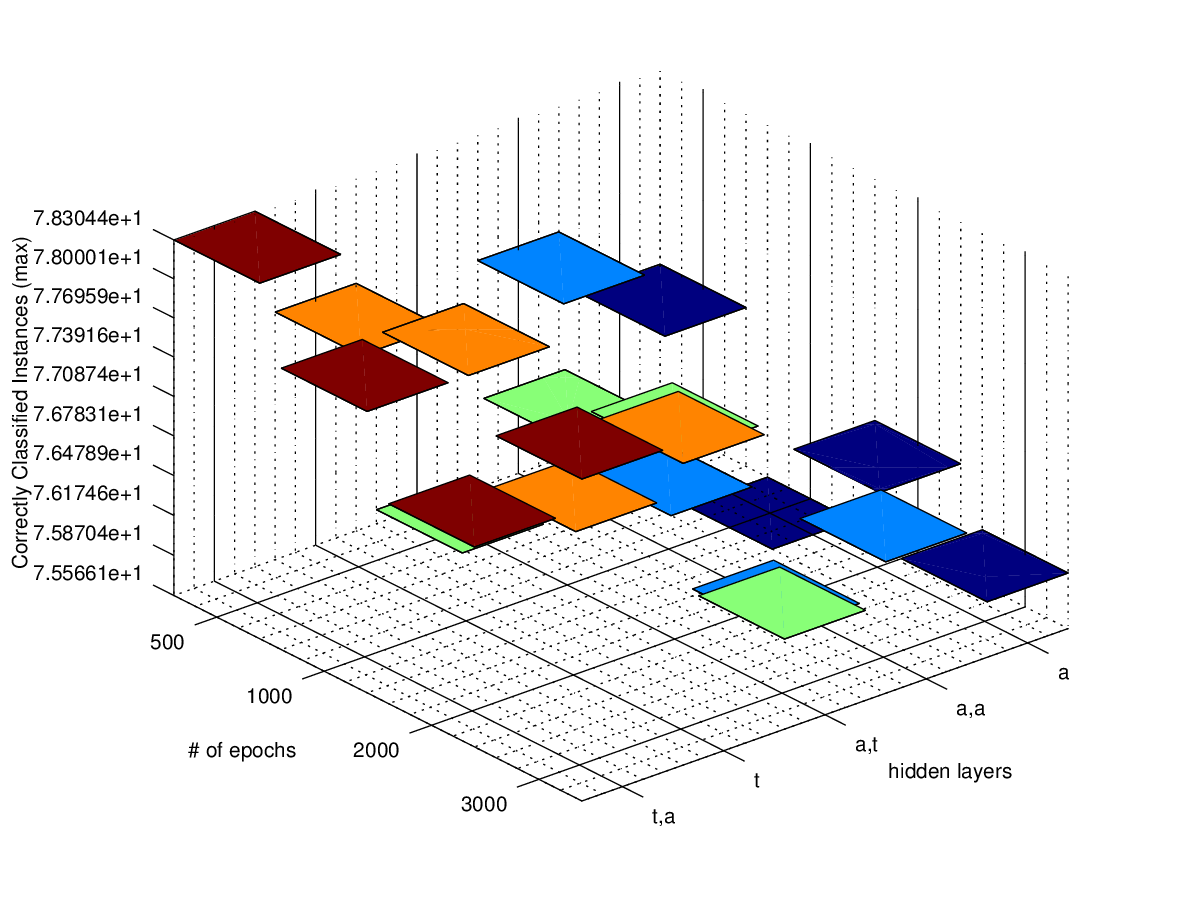
\includegraphics[width=\textwidth]{plots/cmax_NH-log.png}
        \caption{Escala logarítmica.}
        \label{fig:cmax_NH-log}
    \end{subfigure}    
	
	\caption{La proyección del \emph{número de épocas} utilizado y la
			 \emph{configuración de las capas escondidas} 
			 sobre la \textbf{media} (izquierda: \ref{fig:cmean_NH-lin}, \ref{fig:cmean_NH-log})
			 y el \textbf{máximo} (derecha: \ref{fig:cmax_NH-lin}, \ref{fig:cmax_NH-log})
			 del \emph{número de instancias correctamente clasificadas}.}
	\label{fig:NHc}
\end{figure}

\begin{figure}[h]
	\centering
	\begin{subfigure}[b]{0.49\textwidth}
        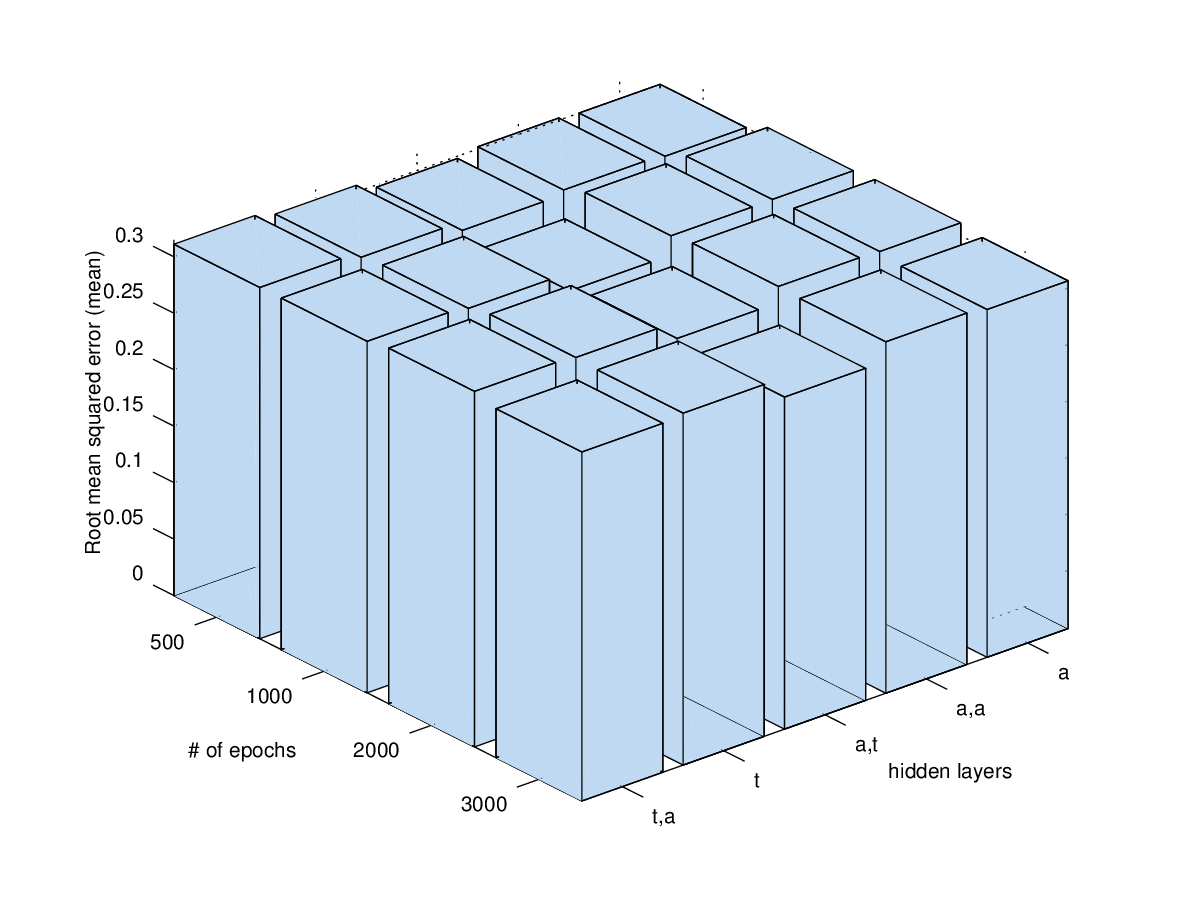
\includegraphics[width=\textwidth]{plots/emean_NH.png}
        \caption{Escala lineal.}
        \label{fig:emean_NH-lin}
    \end{subfigure}
	\begin{subfigure}[b]{0.49\textwidth}
        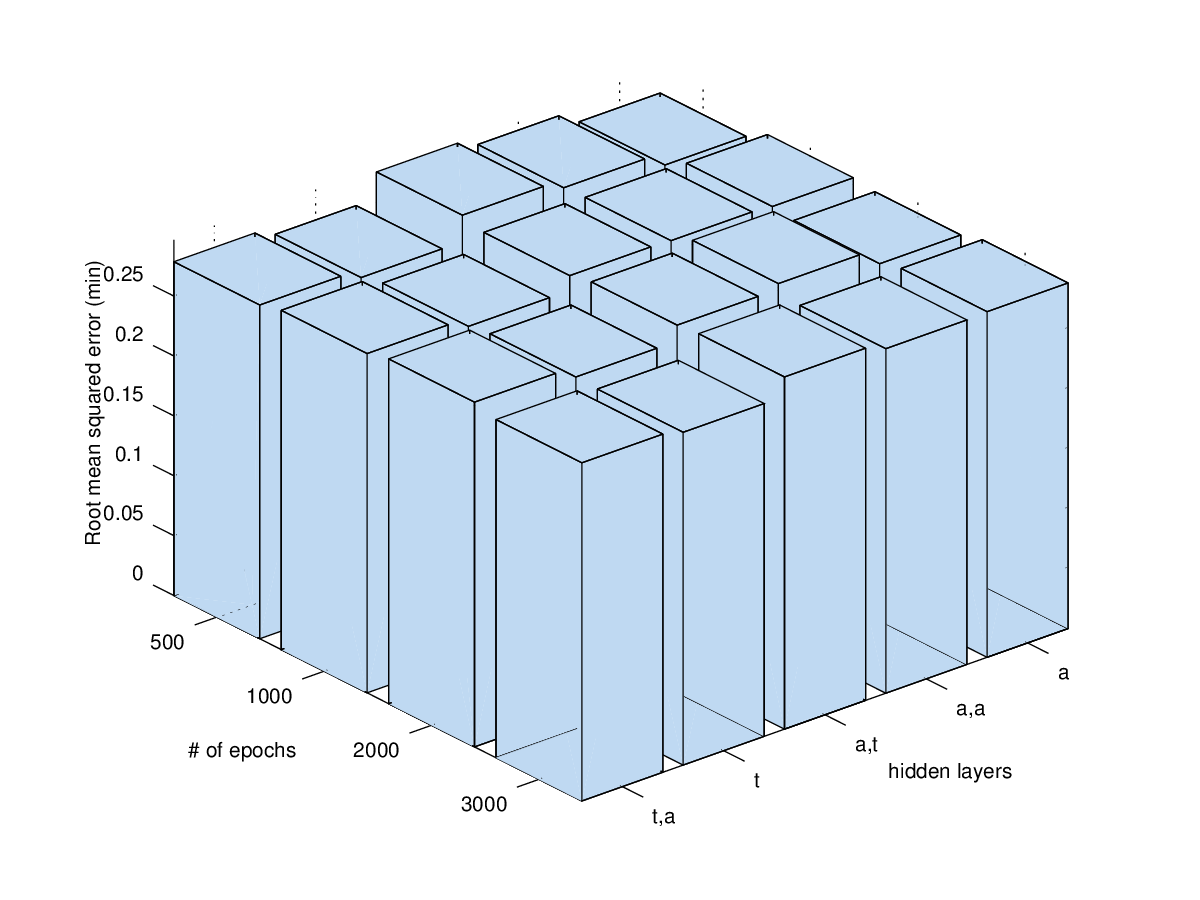
\includegraphics[width=\textwidth]{plots/emin_NH.png}
        \caption{Escala lineal.}
        \label{fig:emin_NH-lin}
    \end{subfigure}
    \\
	\begin{subfigure}[b]{0.49\textwidth}
        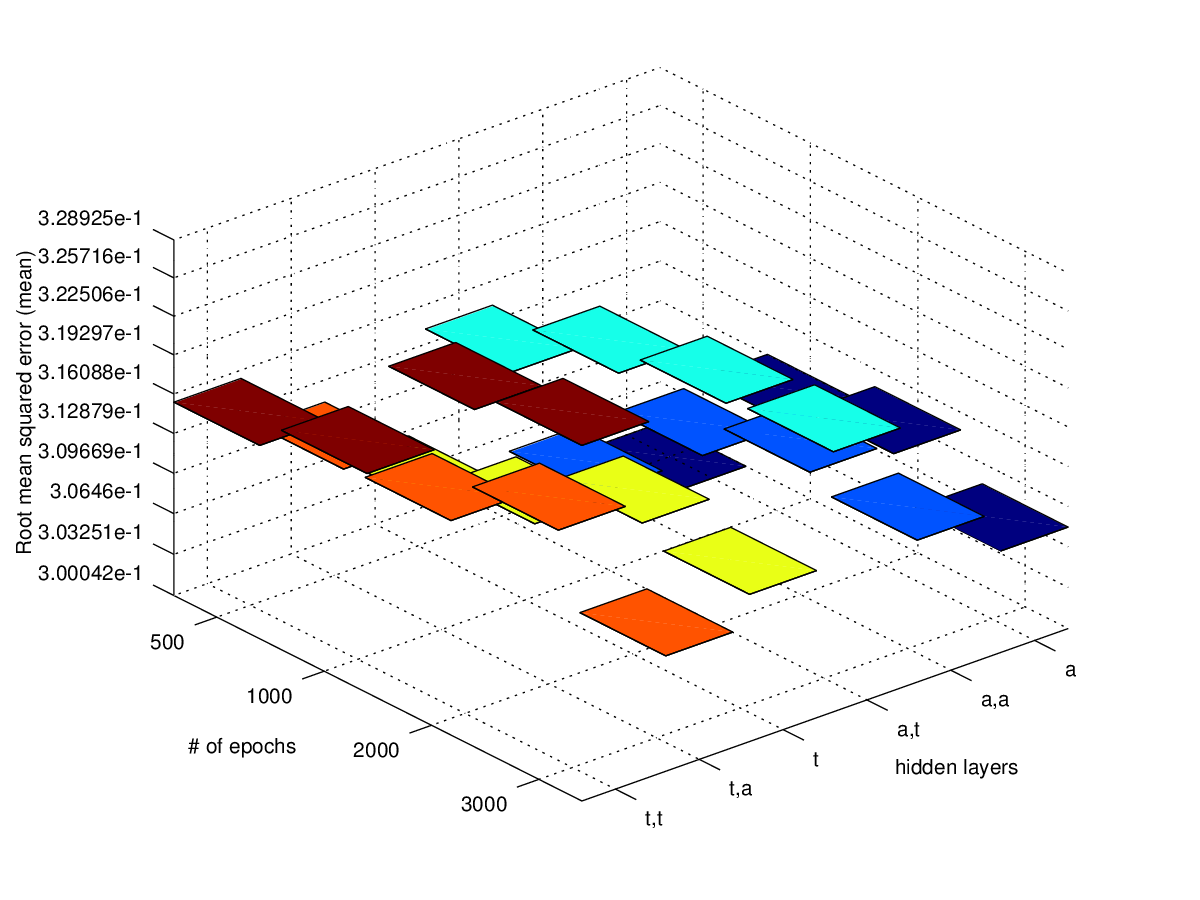
\includegraphics[width=\textwidth]{plots/emean_NH-log.png}
        \caption{Escala logarítmica.}
        \label{fig:emean_NH-log}
    \end{subfigure}
	\begin{subfigure}[b]{0.49\textwidth}
        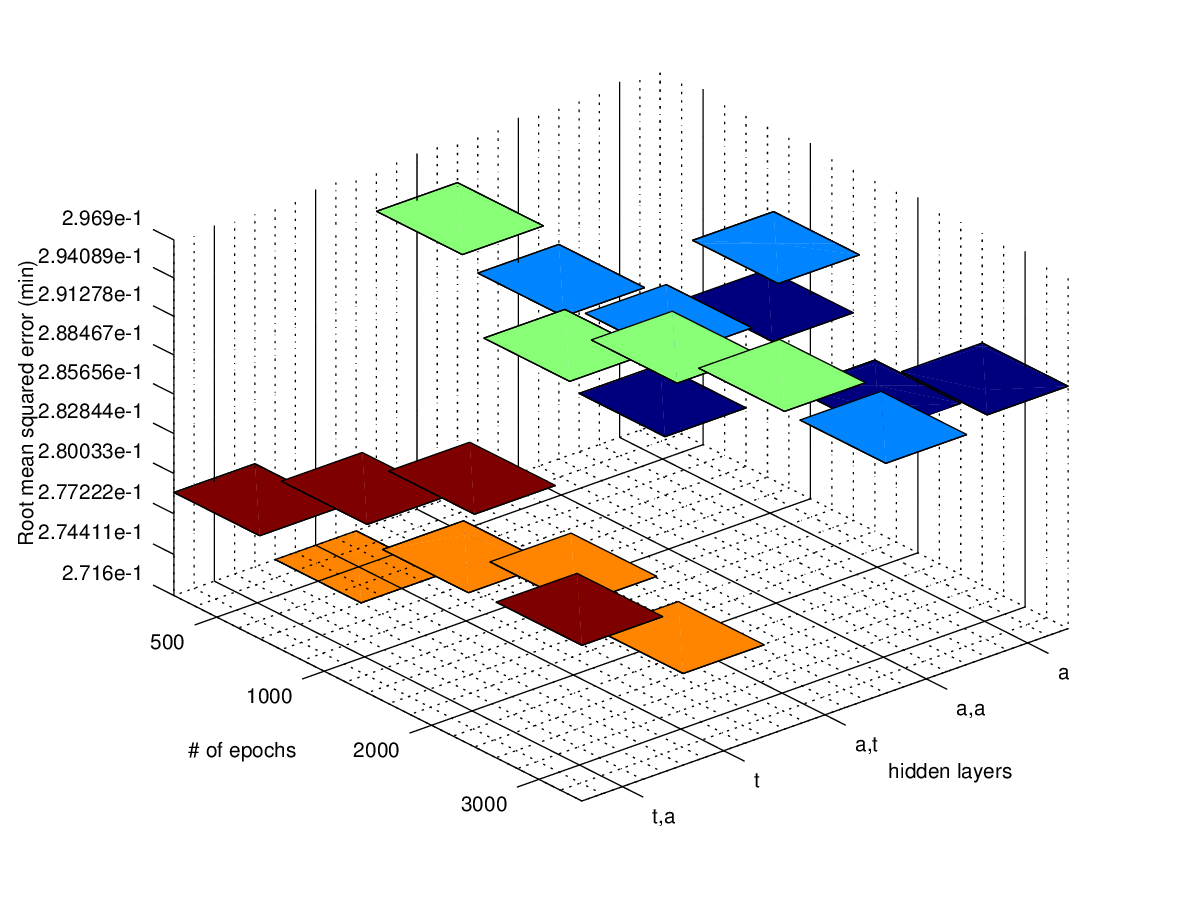
\includegraphics[width=\textwidth]{plots/emin_NH-log.png}
        \caption{Escala logarítmica.}
        \label{fig:emin_NH-log}
    \end{subfigure}    
	
	\caption{La proyección del \emph{número de épocas} utilizado y la
			 \emph{configuración de las capas escondidas} 
			 sobre la \textbf{media} (izquierda: \ref{fig:emean_NH-lin}, \ref{fig:emean_NH-log}) 
			 y el \textbf{mínimo} (derecha: \ref{fig:emin_NH-lin}, \ref{fig:emin_NH-log})
			 de la \emph{error cuadrática media}.}
	\label{fig:NHe}
\end{figure}
	


%\begin{figure}[h]
%	\centering
%	\begin{subfigure}[b]{0.49\textwidth}
%        \includegraphics[width=\textwidth]{plots/.png}
%        \caption{Escala lineal.}
%        \label{fig:-lin}
%    \end{subfigure}
%	\begin{subfigure}[b]{0.49\textwidth}
%        \includegraphics[width=\textwidth]{plots/.png}
%        \caption{Escala lineal.}
%        \label{fig:-lin}
%    \end{subfigure}
%    \\
%	\begin{subfigure}[b]{0.49\textwidth}
%        \includegraphics[width=\textwidth]{plots/-log.png}
%        \caption{Escala logarítmica.}
%        \label{fig:-log}
%    \end{subfigure}
%	\begin{subfigure}[b]{0.49\textwidth}
%        \includegraphics[width=\textwidth]{plots/-log.png}
%        \caption{Escala logarítmica.}
%        \label{fig:-log}
%    \end{subfigure}    
%	
%	\caption{}
%	\label{fig:}
%\end{figure}
